\documentclass[conference]{IEEEtran}
\IEEEoverridecommandlockouts
% The preceding line is only needed to identify funding in the first footnote. If that is unneeded, please comment it out.
\usepackage{cite}
\usepackage{amsmath,amssymb,amsfonts}
\usepackage{algorithmic}
\usepackage{graphicx}
\usepackage{textcomp}
\usepackage{xcolor}
\usepackage{soul}
\def\BibTeX{{\rm B\kern-.05em{\sc i\kern-.025em b}\kern-.08em
    T\kern-.1667em\lower.7ex\hbox{E}\kern-.125emX}}
\usepackage{hyperref}
\hypersetup{
	citecolor = blue,
	linkcolor = blue,
	urlcolor = blue,
	colorlinks = true,
	linkbordercolor = {white}
}


\begin{document}

\title{\textit{CoronaZ}: another distributed systems project
%\\{\footnotesize \textsuperscript{*}Note: Sub-titles are not captured in Xplore and should not be used}
%\thanks{Identify applicable funding agency here. If none, delete this.}
}

\author{
	
	\IEEEauthorblockN{Stefan Ciprian Voinea}
	\IEEEauthorblockA{Università degli Studi di Padova}
	\textit{stefanciprian.voinea@studenti.unipd.it}
	\and
	\IEEEauthorblockN{Name Surname}
	\IEEEauthorblockA{University}
	\textit{mail}
	\and
	\IEEEauthorblockN{Name Surname}
	\IEEEauthorblockA{University}
	\textit{mail}
}

\maketitle

%\begin{abstract}
%This document is a model and instructions for \LaTeX.
%This and the IEEEtran.cls file define the components of your paper [title, text, heads, etc.]. *CRITICAL: Do Not Use Symbols, Special Characters, Footnotes, 
%or Math in Paper Title or Abstract.
%\end{abstract}

%\begin{IEEEkeywords}
%component, formatting, style, styling, insert
%\end{IEEEkeywords}

\section{Introduction}\label{sec:introduction}

	This brief paper describes \textit{CoronaZ}, a project for the Distributed Systems course at the \textit{University of Helsinki}.
	
	All the code of the project is publicly available on GitHub: \textit{\url{https://github.com/cipz/CoronaZ/}}.
	
	This project simulates a contact tracing application where each node represents a person (or a unique device attached to someone) that send signals to each other when in range and communicate the data collected to a server using the \textit{publish-subscribe} pattern.
	The server, called \textit{broker}, can then be polled by a node called \textit{consumer} that will send the data to a database.
	A front-end application then requests this data and displays the movement and the latest updates via the browser.
	
	The idea came from simulating this kind of movements with Arduino boards capable of communicating between them using the \textit{nrf24l01} and to the broker with \textit{esp8266}.
	Unfortunately this was not possible given the relatively strict amount of time that each of the students involved could dedicate to the project and the waiting time to get the necessary hardware.

\section{Technological choices}\label{sec:technological_choices}

	In this section we describe and explain why we have decided to use certain technologies rather than others.
	
	\begin{itemize}
		\item \textit{Programming language}:
		\item \textit{MQTT Broker}:
		\item \textit{Containers}:
		\item \textit{Database}:
		\item \textit{Front-end}:
	\end{itemize}

	\subsection{System requirements}
	
		The system requirements for this project are simple:
		\begin{itemize}
			\item \textit{Docker} and \textit{docker-compose};
			\item Ubuntu or another Linux system for starting the project using the \textit{init-project.sh} bash script;
		\end{itemize}

\section{Architecture}\label{sec:architecture}

	\begin{figure}[htbp]
		\centerline{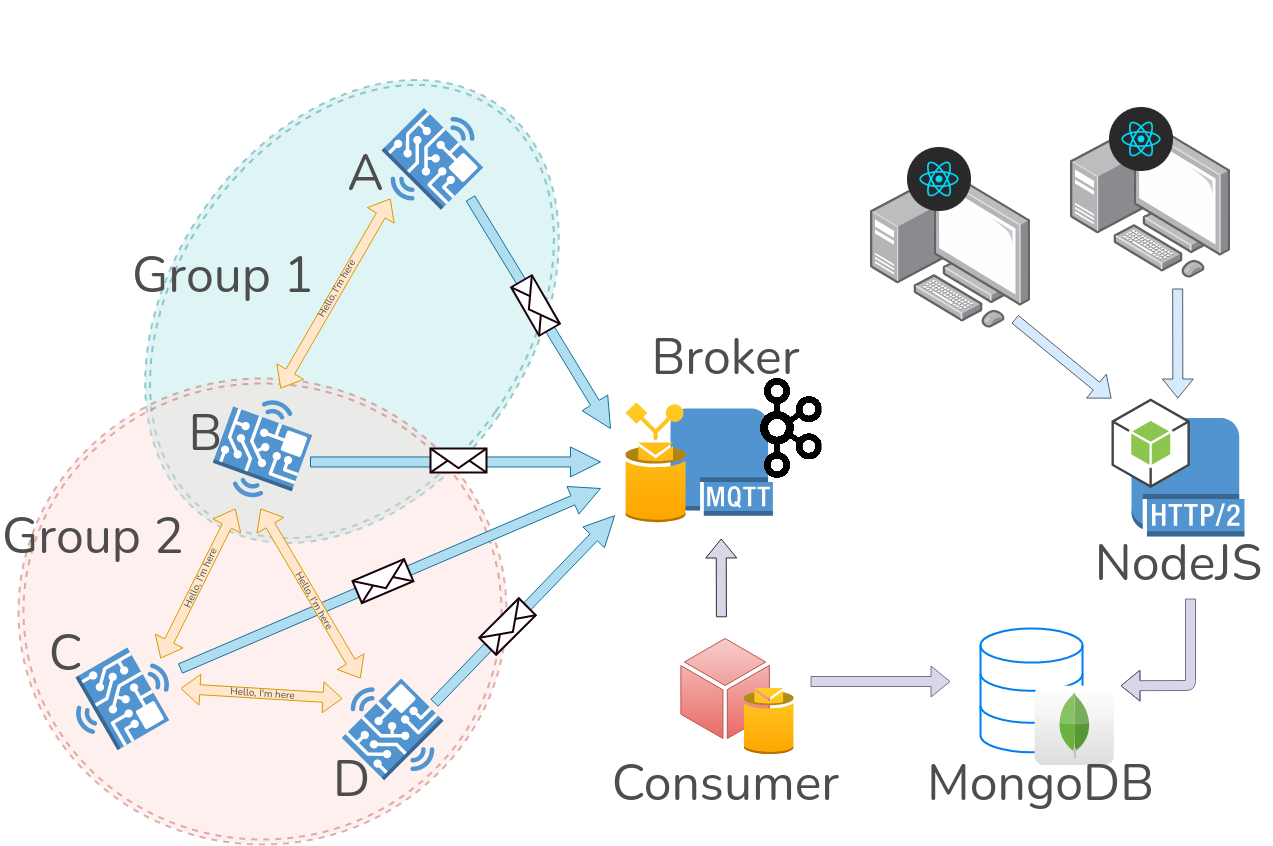
\includegraphics[width=\linewidth]{img/coronaz.png}}
		\caption{Architecture of the \textit{CoronaZ} project.}
		\label{fig:architecture}
	\end{figure}
	
	We can divide our project in four major areas: \textit{nodes}, \textit{broker}, \textit{DB consumer}, \textit{database}, \textit{front-end}.

	\subsection{Nodes}
	
		This can be considered a single area since each node can be spawned separately from one another.
		
		When each node spawns in the map it is placed on a random position.
		
		Every second the node will ``move''.
		When the node moves
		
		Nodes introduced into the simulation can be \textit{infected} or \textit{non-infected} (or \textit{safe}).
		When a node is infected it will keep steady and will not move for a certain amount of time declared in the parameter \texttt{infection\_cooldown}, which defines the number of seconds that the node will stay in place.
		
		In our simulation the nodes can all connect to each other since they are all in the same network and each of them can hear the data sent in broadcast by the others.
		In a more realistic situation nodes would be only capable of hearing the signals of nodes nearby them, like in Fig.\ref{fig:architecture}~where node \textit{A} can communicate only with node \textit{B} and nodes \textit{B}, \textit{C} and \textit{D} are nearby each other enough for them to hear their signal.

	\subsection{MQTT broker}	
	
		Apache Kafka is composed by the Kafka container and the Zookeeper container.
		These can be considered one single 
	
	\subsection{DB consumer}
	
		The DB consumer can be considered as a single entity since it is independent bot from Kafka and from Mongo.
		The consumer is subscribed to the Kafka topic that contains the new messages from the nodes.
		When a new message arrives, the consumer gets it and, every ten messages, it aggregates them in a \texttt{json} that will be sent to the MongoDB database.
	
	\subsection{Database}
	
		MongoDB is the database of our system.
		As the other components it has been containerized in Docker.
		
		It accepts and stores incoming data from the Consumer.
		The database is accessible from the front-end, which will request data every second in order to always display fresh information.
	
%		\begin{figure}[htbp]
%			\centerline{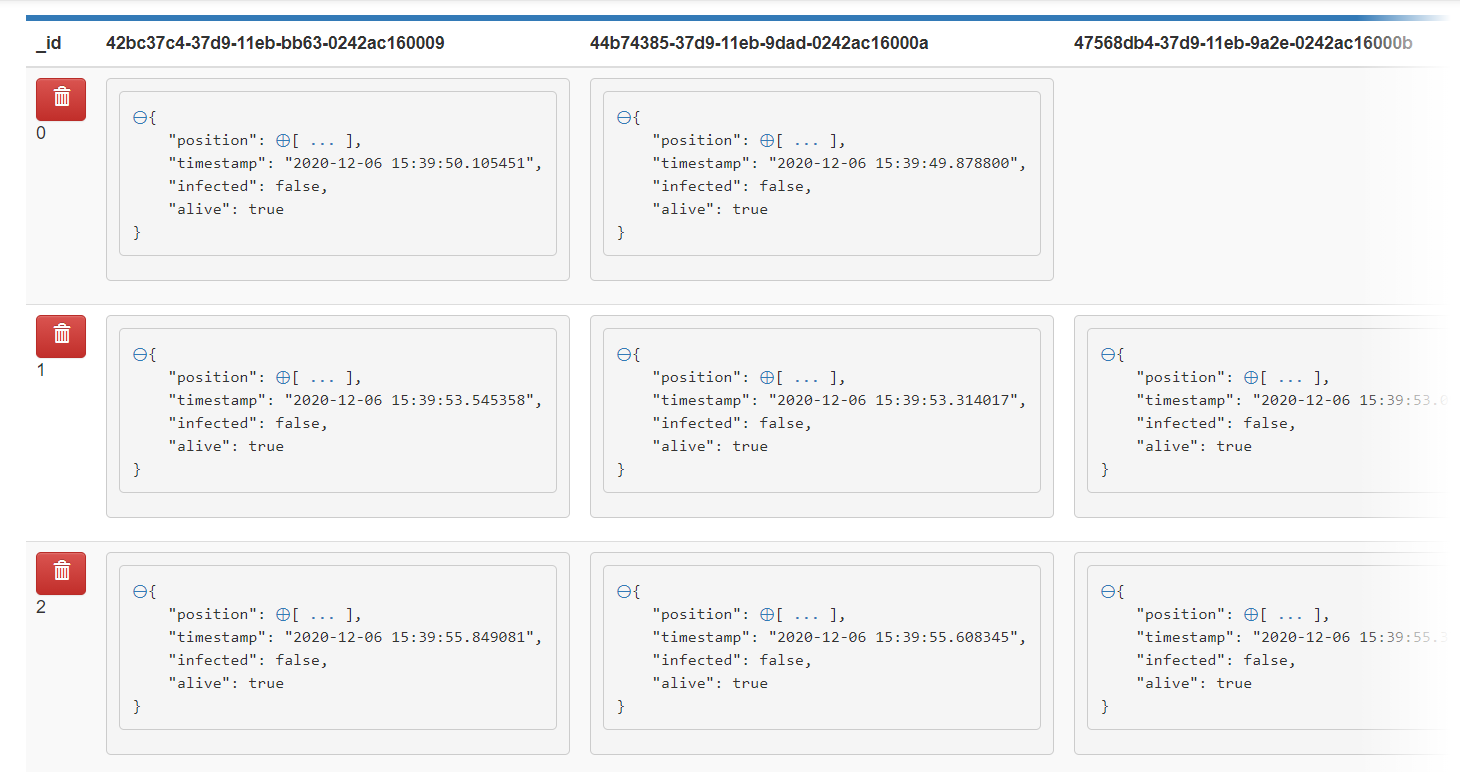
\includegraphics[width=\linewidth]{img/database.png}}
%			\caption{CoronaZ database structure.}
%			\label{fig:database}
%		\end{figure}
	
	\subsection{Front-end}
	
		The front-end of the project, programmed using NodeJS, shows the evolution of the system and the simulation.
		This means that it shows the movement of the nodes in the map, along with which one has been infected or not.
		
%		\begin{figure}[htbp]
%			\centerline{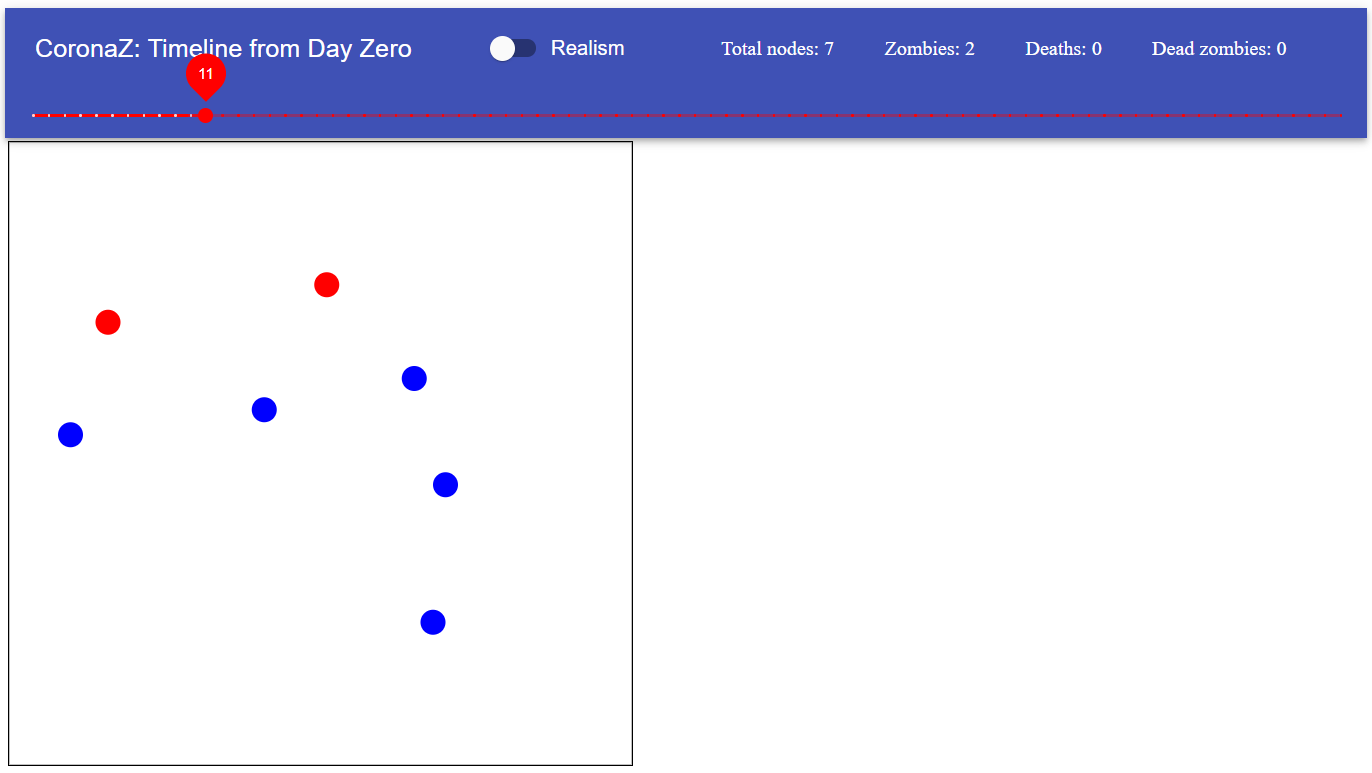
\includegraphics[width=\linewidth]{img/frontend.png}}
%			\caption{CoronaZ front-end.}
%			\label{fig:front-end}
%		\end{figure}

\section{Scalability and fault tolerance}

	We have tested the scalability and the fault tolerance of the project in the following ways:
	
	\begin{itemize}
		\item \textit{unexpectedly shutting down the MongoDB database}:
		\item \textit{unexpectedly shutting down the consumer}:
		\item \textit{unexpectedly shutting down the front end}:
		\item \textit{unexpectedly shutting down the broker}:
		\item \textit{adding more nodes}:
	\end{itemize}
	
\section{Simulation}\label{sec:simulation}

	To start the project we have made a \textit{init-project.sh} script that asks the parameters with which the simulation will take place, that creates the docker network, executes the \texttt{docker-compose} (\texttt{up} and \texttt{down}) commands and manages (and spawns) the number of nodes.
	
%		\begin{figure}[htbp]
%			\centerline{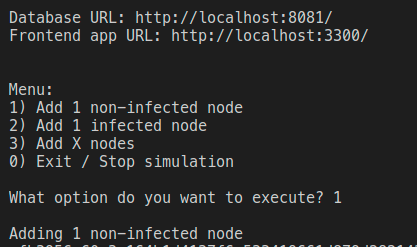
\includegraphics[width=\linewidth]{img/script.png}}
%			\caption{CoronaZ front-end.}
%			\label{fig:front-end}
%		\end{figure}

	The default parameters for the run are (in \textit{json} format):
	\begin{verbatim}
    {
        "field_width" : 100,
        "field_height" : 100,
        "scale_factor" : 5,
        "zombie_lifetime" : 120,
        "infection_radius" : 2,
        "infection_cooldown" : 15
    }
	\end{verbatim}
	
%		\begin{figure}[htbp]
%			\centerline{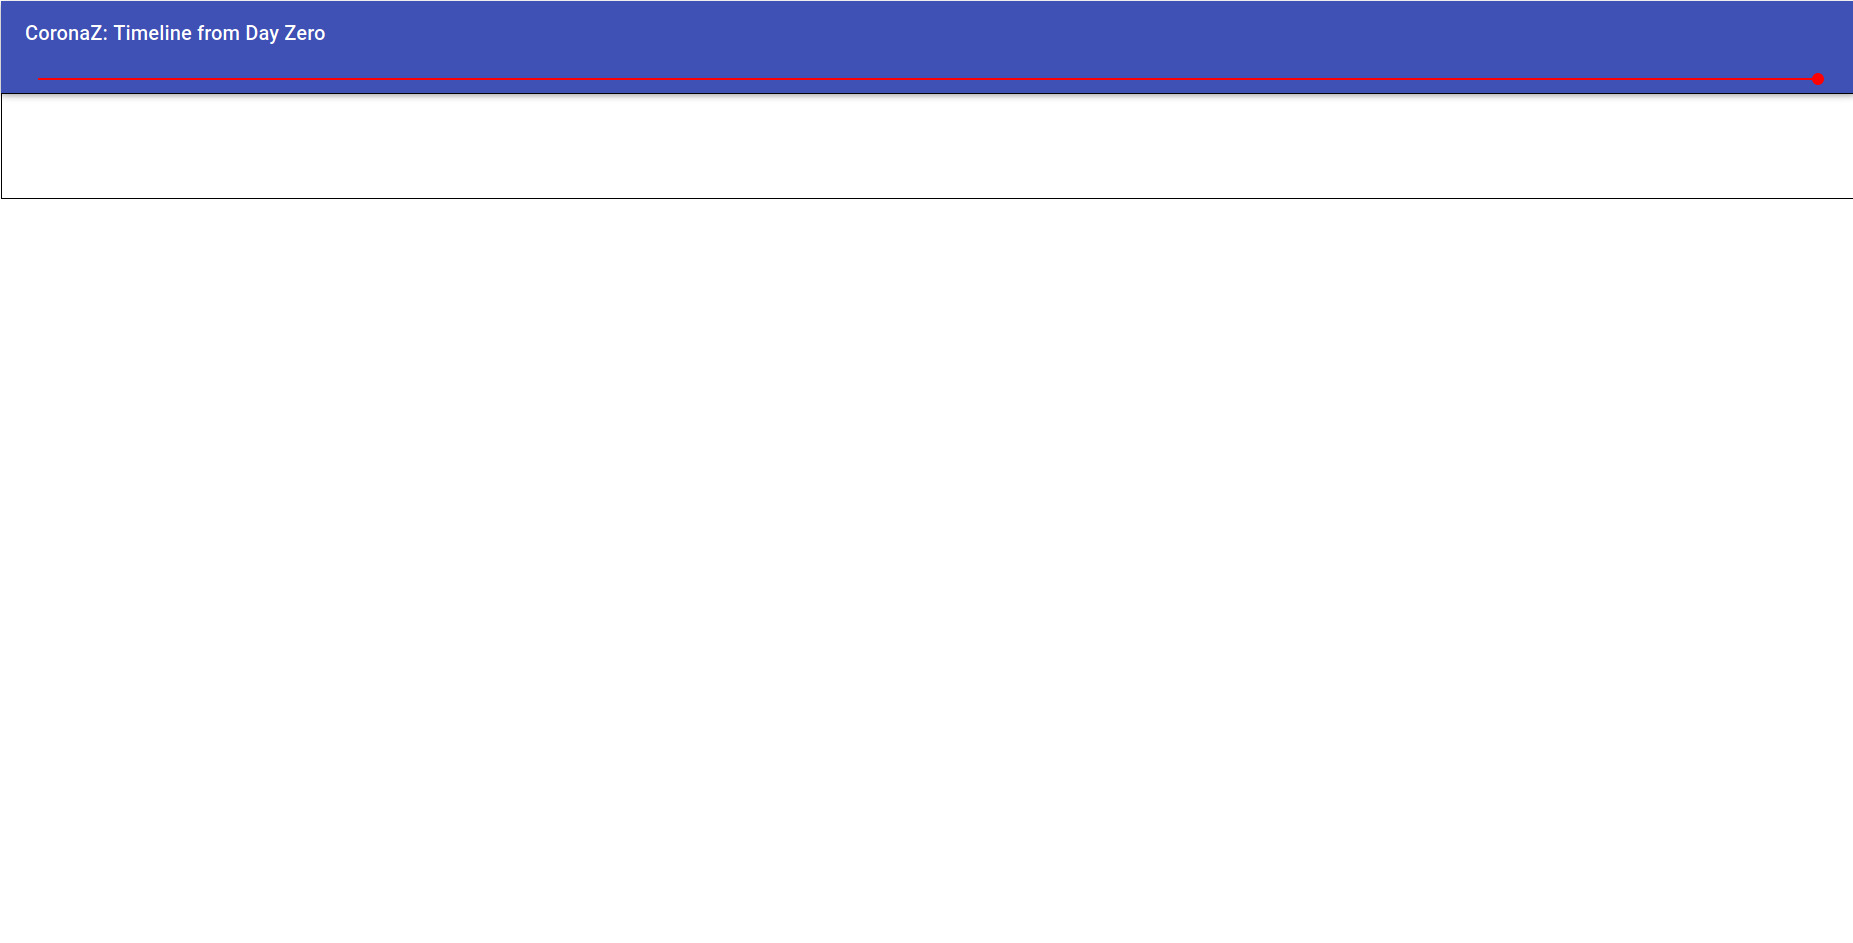
\includegraphics[width=\linewidth]{img/sim_1.png}}
%			\caption{CoronaZ simulation at time X.}
%			\label{fig:sim_1}
%		\end{figure}
%		\begin{figure}[htbp]
%			\centerline{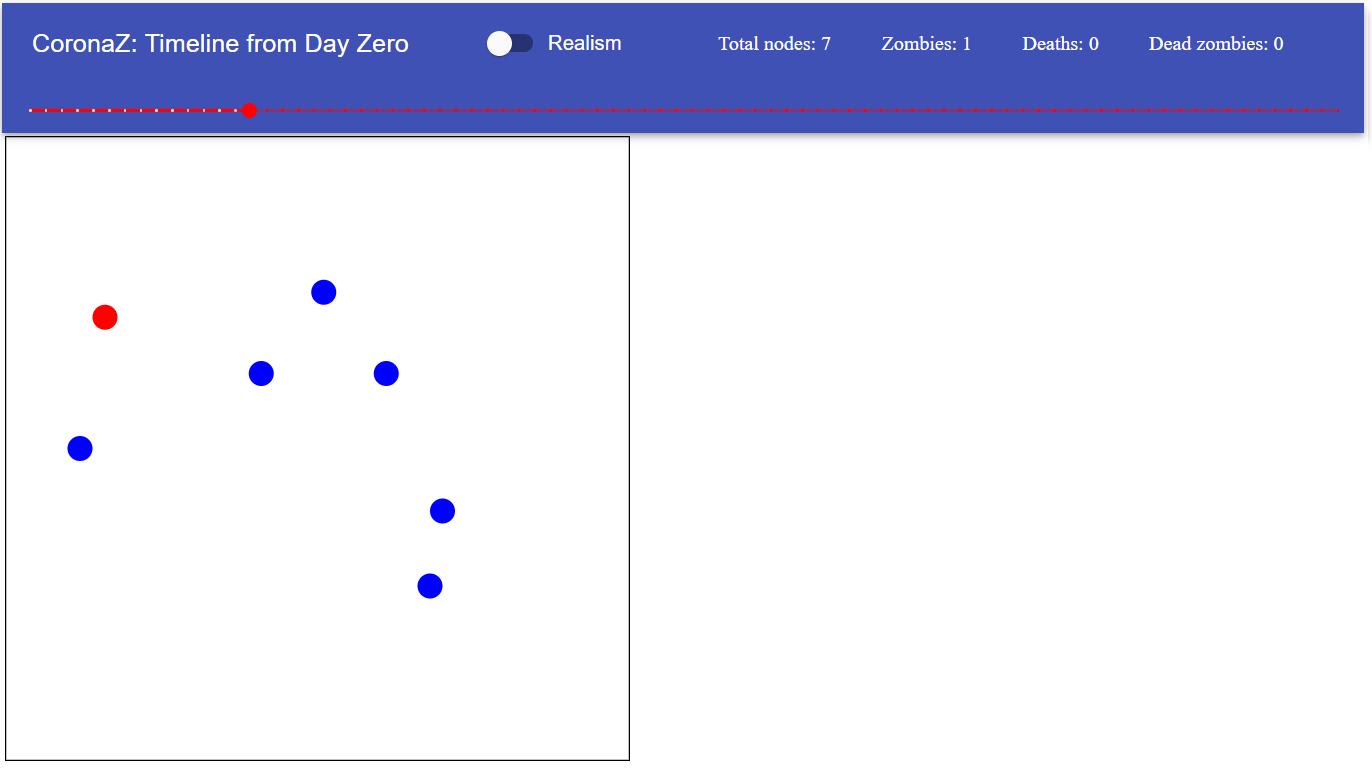
\includegraphics[width=\linewidth]{img/sim_2.png}}
%			\caption{CoronaZ simulation at time X+Y.}
%			\label{fig:sim_2}
%		\end{figure}
%		\begin{figure}[htbp]
%			\centerline{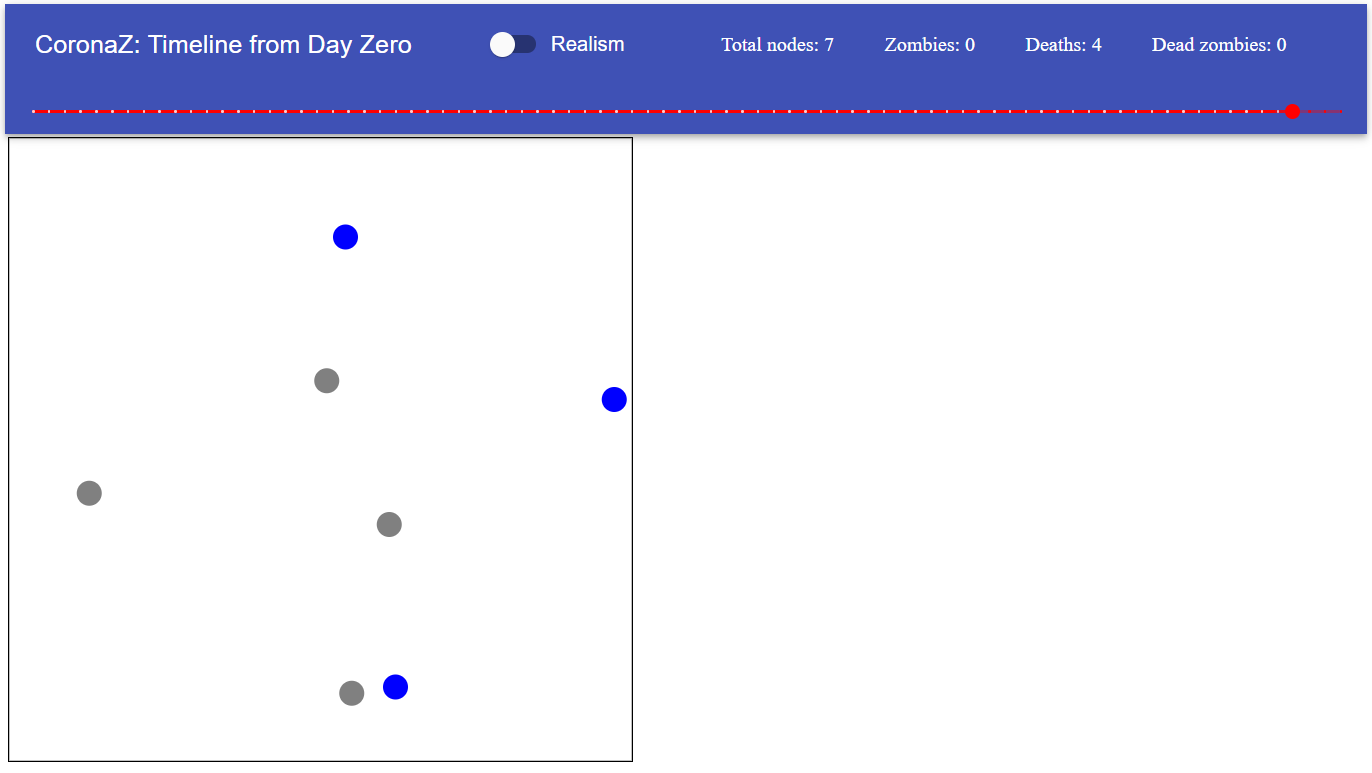
\includegraphics[width=\linewidth]{img/sim_3.png}}
%			\caption{CoronaZ simulation at time X+Y+Z.}
%			\label{fig:sim_3}
%		\end{figure}


\section{Future work}\label{sec:future_work}

	Given the nature of the project there won't be future releases but in this section we want to talk about what can be done to improve the project.
	
	There are various improvements that can be done to make CoronaZ a more interesting and stable simulator, we will tackle them based on the areas defined in \ref{sec:architecture}.
	
\section{Conclusions}\label{sec:conclusions}

	This project represents a simulation of a contact tracing application where each node that spawns in out network communicates its position to the others in range and will send the data collected to a central server with the \textit{publish-subscribe} pattern.

\end{document}
